% Vortragstitel
% hier ist noch kein UTF8 verfügbar, Umlaute mit \"{a} usw. einfügen
\newcommand{\vortragstitel}{Titel (Formatvorlage: Titel; Arial 14 pt, fett, linksbündig)}

% Autor*in/Referent*in
\newcommand{\referent}{Akad. Titel, Vorname, Nachname, Firma, Land des Referenten/der Referentin}

% Co-Autor*innen
\newcommand{\coautoren}{Akad. Titel, Vorname, Nachname, Firma, Land des Co-Autors/der Co-Autorin\\
ggf. weitere Co-Autor*innen darunter mit den gleichen Angaben, jeweils in neuer Zeile\\
(Formatvorlage: Autor*innen; Arial 11 pt, linksbündig)}

% Schlüsselwörter
\newcommand{\schluesselwoerter}{Modenverwirbelungskammer, Reverberation Chamber, Statistische Verteilung, Korrelation, Leitungstheorie, Störfestigkeitsuntersuchung, Elektromagnetische Verträglichkeit, Richtwirkung, Direktivität, Absorberhalle, Wellenleiter, Prüflingsmodell}

% zentrale Einstellungen laden
\input{Einstellungen}

% ab hier ist UTF8 verfügbar und Umlaute können ganz normal geschrieben werden
\section{Hauptüberschrift 1 (Formatvorlage: Überschrift 1; Arial 11 pt, fett, linksbündig)}

Beginnen Sie hier mit dem Paper (Formatvorlage: Standard; Arial 11 pt, Blocksatz). Grafiken, Tabellen etc. können ebenfalls hier eingefügt werden.

Quellenangaben lassen sich via \verb|\cite{}|-Befehl einfügen und müssen dazu in der \texttt{literatur.bib}-Datei eingetragen sein.

\nocite{quelle1,quelle2,quelle3,quelle4,quelle5}

Weitere Informationen zum Angeben von Quellen sind im IEEE Reference Guide~\cite{ieee:style_manual} zu finden.

Abschließend wird auf die exemplarische Tabelle~\ref{tab:beispiel} verwiesen.

\begin{table}
	\centering
		\begin{tabular}{@{}p{0.45\textwidth}p{0.45\textwidth}@{}}
			\toprule
			\bfseries Überschrift der Tabellenspalte & \bfseries Überschrift der Tabellenspalte \\
			\midrule
			Tabelleninhalt & Tabelleninhalt \\
			\midrule
			Tabelleninhalt & Tabelleninhalt \\
			\midrule
			Tabelleninhalt & Tabelleninhalt \\
			\bottomrule
	\end{tabular}
	\caption{Beispiel einer Tabellenunterschrift}
	\label{tab:beispiel}
\end{table}
 
Ein beispielhafter Messaufbau ist in Abbildung~\ref{fig:aufbau} gezeigt.

\begin{figure}
	\centering
		\begin{tikzpicture}
			% Signalgenerator
			\node[draw] (sg) {Signalgenerator};
			% Spektrumanalysator
			\node[draw,right=of sg] (sa) {Spektrumanalysator};
			% Verbindungspfeil
			\draw[->] (sg) -- (sa);
		\end{tikzpicture}
	\caption{Messaufbau (Bildunterschrift in Arial 10 pt, linksbündig, bei viel Text Blocksatz)}
	\label{fig:aufbau}
\end{figure}

Ein beispielhaftes Messergebnis ist in Abbildung~\ref{fig:ergebnis} dargestellt.

\begin{figure}
	\centering
		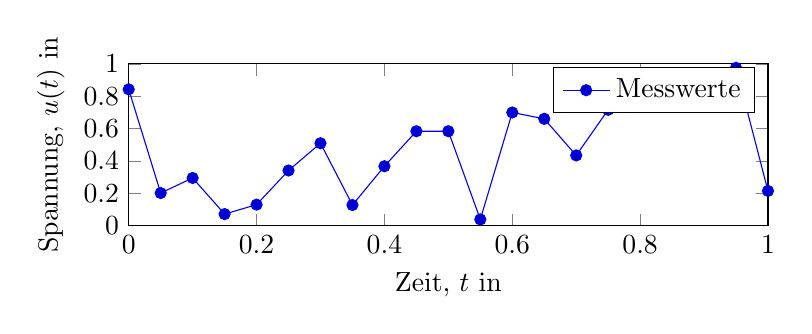
\begin{tikzpicture}
			\begin{axis}[
				xlabel={Zeit, $t$ in \si{\second}},
				ylabel={Spannung, $u(t)$ in \si{\volt}},
				width=0.8\textwidth,
				height=0.3\textwidth,
				xmin=0,xmax=1,
				ymin=0,ymax=1,
				]
				\addplot+[
					domain=0:1,
					samples=21,
				]{rnd};
				\addlegendentry{Messwerte}
			\end{axis}
		\end{tikzpicture}
	\caption{Messergebnis (Bildunterschrift in Arial 10 pt, linksbündig, bei viel Text Blocksatz)}
	\label{fig:ergebnis}
\end{figure}

%Eine beispielhafte tabellarische Aufstellung ist in Tabelle~\ref{tab:beispieltabelle} gezeigt.
%
%\begin{table}
	%\centering
		%\begin{tabular}{@{}p{0.15\textwidth}p{0.15\textwidth}p{0.15\textwidth}p{0.15\textwidth}p{0.15\textwidth}@{}}
			%\toprule
			%Lorem & Ipsum & Dolor & Sit & Amet \\
			%\midrule
			%consectetuer & sed diam & sed diam & sed diam & sed diam \\
			%\midrule
			%adipiscing & sed diam & sed diam & sed diam & sed diam \\
			%\midrule
			%elit & sed diam & sed diam & sed diam & sed diam \\
			%\bottomrule
	%\end{tabular}
	%\caption{Beispieltabelle (Arial 10 pt, linksbündig, bei viel Text Blocksatz)}
	%\label{tab:beispieltabelle}
%\end{table}

Nachfolgend werden noch Beispiele für Überschriften gezeigt. Viel Erfolg für Ihr Schreibprojekt!

\subsection{Untertitel 1 (Formatvorlage: Überschrift 2; Arial 11 pt, fett, linksbündig)}

Hier können Sie Zwischenthemen einfügen (Formatvorlage: Standard; Arial 11 pt, Blocksatz).

%\blindtext

\subsubsection{Untertitel 2 (Formatvorlage: Überschrift 3; Arial 11 pt, linksbündig)}

%Text zum weiteren Unterpunkt (Arial 11 pt, Blocksatz).

\paragraph{Untertitel 3 (Formatvorlage: Überschrift 4; Arial 11 pt, linksbündig, kursiv)}

Text zum weiteren Unterpunkt (Formatvorlage: Standard; Arial 11 pt, Blocksatz).

\section{Hinweise zu den Formatvorlagen der Beschriftungen}

Die Beschriftung der Abbildungen sind wie nachfolgend zu formatieren:

\begin{figure}
	\caption{Bildunterschrift (Formatvorlage: Beschriftung; Arial 10 pt, linksbündig, bei viel Text Blocksatz)}
\end{figure}

Tabellen sind wie nachfolgend dargestellt zu beschriften:

\begin{table}
	\caption{Tabellenunterschrift (Formatvorlage: Beschriftung; Arial 10 pt, linksbündig, bei viel Text Blocksatz)}
\end{table}

% die Literaturliste mit BibTeX
% als PDF-Lesezeichen hinzufügen
%\pdfbookmark{\refname}{Literatur}
%\bibliographystyle{plaindin}	% nur Nummern, nach DIN
%\bibliographystyle{ieeetran}	% nur Nummern, nach IEEE
%\bibliography{literatur}
% die Literaturliste mit biblatex
\printbibliography

\end{document}
